\documentclass[12pt,a4paper]{article}
% Packages
\usepackage[utf8]{inputenc}
\usepackage[T1]{fontenc}
\usepackage{amsmath,amssymb}
\usepackage{graphicx}
\usepackage[hidelinks]{hyperref}
\usepackage{authblk} % Package for multiple authors
\usepackage{booktabs} % For better tables
\usepackage{listings} % For code snippets
\usepackage{xcolor} % For colored text
\usepackage{float} % For better figure placement with [H]
% Define Prolog language style for listings
\definecolor{prologcomment}{rgb}{0.5,0.5,0.5} % Gray for comments
\definecolor{prologkeyword}{rgb}{0,0,0.8} % Blue for keywords/predicates
\definecolor{prologstring}{rgb}{0.8,0,0} % Red for strings/atoms
\definecolor{prologvariable}{rgb}{0,0.5,0} % Green for variables
\lstdefinestyle{prologstyle}{
language=Prolog,
basicstyle=\ttfamily\small,
keywordstyle=\color{prologkeyword}\bfseries,
commentstyle=\color{prologcomment},
stringstyle=\color{prologstring},
identifierstyle=\color{prologvariable}, % Style for variables
morekeywords={node, arc, edge, find\_simple\_cycles, generate\_edges, find\_all\_elementary\_cycles, dfs\_find\_cycle, filter\_simple\_cycles, is\_simple\_cycle, check\_all\_pairs\_shortest\_path, check\_pairs\_from\_node, get\_cycle\_distance, shortest\_path\_length, bfs, add\_neighbors\_to\_queue, normalize\_cycle, find\_min\_node, rotate\_list\_to\_start\_with, print\_cycles\_list, print\_cycles\_list\_reversed, member, length, writeln, write, nl, retractall, forall, assertz, findall, reverse, append, nth0, list\_to\_set, setof, main, setup\_test, read, halt}, % Added new main predicates
morecomment=[l]{//}, % Line comments starting with //
morecomment=[l]{\%}, % Line comments starting with %
morestring=[b]', % Single quoted strings/atoms
morestring=[b]", % Double quoted strings (less common in Prolog)
showstringspaces=false,
tabsize=2,
breaklines=true,
breakatwhitespace=true,
captionpos=b, % Position caption below the listing
frame=single % Add a frame around the code
}
% Title and author information
\title{Finding Simple Cycles in a Directed Graph using Prolog}
\author[1]{Cirilli Davide}
\author[2]{Fontana Emanuele}
\affil[1,2]{Department of Computer Science, Università degli Studi di Bari}
\begin{document}
\maketitle
\begin{abstract}
This document describes a Prolog program designed to identify all "simple cycles" within a directed graph. The program features an interactive main predicate that allows selection from predefined test cases. For a chosen graph, it first finds all elementary cycles and then filters them based on a specific shortest path criterion to determine simplicity. The implementation utilizes Depth-First Search (DFS) for cycle detection and Breadth-First Search (BFS) for shortest path calculations.
\end{abstract}
\tableofcontents
\section{Introduction}
A cycle in a directed graph is a path that starts and ends at the same node. An \textit{elementary cycle} is a cycle where no node (except the start/end node) appears more than once. This program aims to find a subset of elementary cycles termed "simple cycles".
A cycle is defined as \textit{simple} if, for any two distinct nodes 
$u$ 
 and 
$v$ 
 within the cycle, the shortest path from 
$u$ 
 to 
$v$ 
 in the \textit{entire graph} is the path that follows the edges of the cycle itself. If a shorter path (a "shortcut") exists between 
$u$ 
 and 
$v$ 
 using edges outside the cycle, the cycle is not considered simple.
This program implements this definition using Prolog, leveraging its backtracking capabilities for graph traversal and dynamic fact manipulation for setting up different graph structures.
\section{Implementation Details}
The Prolog program (\texttt{simpleCycle.pl}) begins with directives:
\begin{verbatim}
:- dynamic node/2.
:- dynamic arc/4.
:- dynamic edge/2.
\end{verbatim}
The \texttt{:- dynamic Predicate/Arity} directive declares that facts for \texttt{node/2}, \texttt{arc/4}, and the helper \texttt{edge/2} can be added (\texttt{assertz}) or removed (\texttt{retractall}) during program execution. This is crucial for the \texttt{setup\_test/1} predicate, which defines different graph structures, and for \texttt{generate\_edges/0}, which dynamically creates \texttt{edge/2} facts.
The program consists of several key components:
\subsection{Graph Representation and Setup}
The graph is primarily defined by \texttt{arc/4} facts, which are dynamically asserted by test case setup predicates.
\begin{itemize}
\item \texttt{node(NodeID, Type)}: Declares a node with a unique ID and an associated type. While test cases primarily define connectivity through \texttt{arc/4} facts, default \texttt{node/2} facts are provided in the code. These are used by \texttt{find\_all\_elementary\_cycles/1} to gather an initial list of all potential starting nodes for cycle detection.
\item \texttt{arc(ArcID, Type, SourceNode, TargetNode)}: Declares a directed arc with a unique ID, type, source node, and target node. These facts define the graph's structure for a given test case.
\item \texttt{setup\_test/1}: A predicate responsible for configuring the graph for a chosen test case (1, 2, 3, or 4). It first calls \texttt{retractall(arc(\_, \_, \_, \_))} to clear any existing arc definitions and then asserts the specific \texttt{arc/4} facts for the selected test case.
\end{itemize}
For traversal efficiency, a helper predicate \texttt{edge(Source, Target)} is dynamically generated from the current \texttt{arc/4} facts.
\begin{itemize}
\item \texttt{generate\_edges/0}: This predicate prepares the graph for traversal.
\begin{itemize}
\item It first calls \texttt{retractall(edge(\_, \_))} to remove any existing \texttt{edge/2} facts, ensuring a clean state corresponding to the current set of \texttt{arc/4} facts.
\item Then, \texttt{forall(arc(\_, \_, N, M), assertz(edge(N, M)))} iterates through all current \texttt{arc/4} facts. For each, it extracts the source (\texttt{N}) and target (\texttt{M}) nodes and asserts a new fact \texttt{edge(N, M)}. This provides faster lookups for direct connections.
\end{itemize}
\end{itemize}
\subsection{Finding Elementary Cycles}
Elementary cycles are found using a Depth-First Search (DFS) approach:
\begin{itemize}
\item \texttt{find\_all\_elementary\_cycles/1}: The main predicate for this stage.
\begin{itemize}
\item It uses \texttt{findall(N, node(N, \_), Nodes)} to collect all \texttt{NodeID}s from the currently asserted \texttt{node/2} facts into the list \texttt{Nodes}. These nodes serve as potential starting points for cycles.
\item It then calls \texttt{find\_cycles\_starting\_from\_nodes/2} with this list.
\item The argument \texttt{Cycles} will be unified with the list of all elementary cycles found.
\end{itemize}
\item \texttt{find\_cycles\_starting\_from\_nodes/2}: Iterates through all nodes from the \texttt{Nodes} list and initiates DFS from each.
\begin{itemize}
\item It uses \texttt{findall/3}. The template is \texttt{Cycle}.
\item The goal is \texttt{(member(StartNode, Nodes), edge(StartNode, Neighbor), dfs\_find\_cycle(Neighbor, StartNode, [Neighbor, StartNode], Cycle))}.
\item \texttt{member(StartNode, Nodes)} iterates through each node as a potential starting point.
\item \texttt{edge(StartNode, Neighbor)} finds a node directly reachable from \texttt{StartNode}.
\item \texttt{dfs\_find\_cycle/4} is called to perform DFS starting from this \texttt{Neighbor}, aiming to return to \texttt{StartNode}. The path is initialized with \texttt{[Neighbor, StartNode]}.
\item \texttt{findall/3} collects all \texttt{Cycle} bindings found through backtracking.
\end{itemize}
\item \texttt{dfs\_find\_cycle/4}: Performs the recursive DFS: \texttt{dfs\_find\_cycle(CurrentNode, TargetNode, PathSoFar, Cycle)}.
\begin{itemize}
\item It looks for an edge from \texttt{CurrentNode} to \texttt{NextNode} using \texttt{edge(CurrentNode, NextNode)}.
\item Base Case: If \texttt{NextNode == TargetNode}, the starting node is reached. \texttt{Cycle} is unified with \texttt{[TargetNode | PathSoFar]}.
\item Recursive Step: If \texttt{NextNode} is not \texttt{TargetNode}, it checks \texttt{\textbackslash+ memberchk(NextNode, PathSoFar)} to ensure elementarity. If not visited in the current path, it recursively calls \texttt{dfs\_find\_cycle(NextNode, TargetNode, [NextNode | PathSoFar], Cycle)}.
\end{itemize}
\item Cycles from DFS are returned in reverse traversal order (e.g., \texttt{[a, d, c, b, a]} for a cycle $a \rightarrow b \rightarrow c \rightarrow d \rightarrow a$). 
\end{itemize}
\subsection{Filtering for Simple Cycles}
The logic for identifying simple cycles:
\begin{itemize}
\item \texttt{filter\_simple\_cycles/2}: Takes \texttt{ElementaryCycles} and returns \texttt{NormalizedSimpleCycles}.
\begin{itemize}
\item Base Case: \texttt{filter\_simple\_cycles([], [])}.
\item Recursive Step 1 (Simple Cycle Found): If \texttt{is\_simple\_cycle(Cycle)} succeeds for the head \texttt{Cycle}, it's cut (\texttt{!}), normalized via \texttt{normalize\_cycle(Cycle, NormalizedCycle)}, and prepended to the result of recursively processing \texttt{RestCandidates}.
\item Recursive Step 2 (Not Simple): If \texttt{is\_simple\_cycle(Cycle)} fails, the \texttt{\_Cycle} is ignored, and the predicate recurses on \texttt{RestCandidates}.
\end{itemize}
\item \texttt{is\_simple\_cycle/1}: Checks if an elementary cycle is simple.
\begin{itemize}
\item Reverses the DFS cycle: \texttt{reverse(Cycle, ForwardCycleWithRepeatEnd)}.
\item Deconstructs to get ordered unique nodes: \texttt{ForwardCycleWithRepeatEnd = [StartNode | PathNodesWithRepeatEnd]}, \texttt{append(PathNodesUnique, [StartNode], PathNodesWithRepeatEnd)}, \texttt{NodesInCycleOrdered = [StartNode | PathNodesUnique]}. E.g., for DFS output \texttt{[a,c,b,a]}, this yields \texttt{[a,b,c]}.
\item Calls \texttt{check\_all\_pairs\_shortest\_path(NodesInCycleOrdered, NodesInCycleOrdered)}.
\end{itemize}
\item \texttt{check\_all\_pairs\_shortest\_path/2}: Iterates through ordered pairs $(u,v)$ 
 in \texttt{NodesInCycleOrdered}.
\begin{itemize}
\item Base Case: \texttt{check\_all\_pairs\_shortest\_path([], \_)}.
\item Recursive Step: Takes \texttt{N1} from the list, calls \texttt{check\_pairs\_from\_node(N1, OriginalCycleNodes, OriginalCycleNodes)}, then recurses on \texttt{RestN1}.
\end{itemize}
\item \texttt{check\_pairs\_from\_node/3}: For a given \texttt{N1}, iterates through other nodes \texttt{N2} in \texttt{OriginalCycleNodes}.
\begin{itemize}
\item Base Case: \texttt{check\_pairs\_from\_node(\_, [], \_)}.
\item Recursive Step: Takes \texttt{N2}.
\item If \texttt{N1 == N2}, skip (\texttt{true}).
\item Else, calculate \texttt{get\_cycle\_distance(N1, N2, OriginalCycleNodes, CycleDist)} and \texttt{shortest\_path\_length(N1, N2, ShortestDist)}.
\item Check simplicity:
\begin{itemize}
\item If \texttt{ShortestDist == -1} (no path in graph), then $CycleDist > 0$ 
 must hold (or \texttt{!, fail}).
\item Else (path exists), $ShortestDist \ge CycleDist$ 
 must hold.
\end{itemize}
\item If the check succeeds, cut (\texttt{!}) and recurse on \texttt{RestN2}.
\item Failure Clause: \texttt{check\_pairs\_from\_node(\_, \_, \_) :- !, fail.} ensures immediate failure if any pair violates simplicity.
\end{itemize}
\item \texttt{get\_cycle\_distance/4}: Calculates distance from \texttt{NodeA} to \texttt{NodeB} along \texttt{CycleNodes}.
\begin{itemize}
\item Finds indices \texttt{IndexA}, \texttt{IndexB} using \texttt{nth0/3}. Gets \texttt{length(CycleNodes, Len)}.
\item If $IndexB \ge IndexA$, $Distance = IndexB - IndexA$. 
\item Else, $Distance = Len - IndexA + IndexB$. 
\end{itemize}
\item \texttt{shortest\_path\_length/3}: Finds shortest path length between \texttt{Start} and \texttt{End} using BFS.
\begin{itemize}
\item Calls \texttt{bfs([[Start, 0]], End, [Start], Length)}.
\item Cuts (\texttt{!}) on success. If BFS fails, the second clause \texttt{shortest\_path\_length(\_, \_, -1)} sets \texttt{Length} to -1.
\end{itemize}
\item \texttt{bfs/4}: Standard BFS: \texttt{bfs(Queue, Target, Visited, Length)}.
\begin{itemize}
\item Base Case 1 (Queue Empty): \texttt{bfs([], \_, \_, \_) :- !, fail.}
\item Base Case 2 (Target Found): \texttt{bfs([[Target, Length] | \_], Target, \_, Length) :- !.}
\item Recursive Step: Dequeues \texttt{[Current, Dist]}. Finds unvisited neighbors via \texttt{findall(Next, (edge(Current, Next), \textbackslash+ member(Next, Visited)), Neighbors)}. Calculates $NewDist = Dist + 1$. 
 Adds neighbors to queue via \texttt{add\_neighbors\_to\_queue/4}. Updates visited list (using \texttt{append/3} and \texttt{list\_to\_set/2}). Recurses.
\end{itemize}
\item \texttt{add\_neighbors\_to\_queue/4}: Formats neighbors as \texttt{[Node, Distance]} and appends to queue using \texttt{findall/3} and \texttt{append/3}.
\end{itemize}
\subsection{Cycle Normalization}
Ensures unique representation for identical cycles starting at different nodes.
\begin{itemize}
\item \texttt{normalize\_cycle/2}: Converts raw DFS cycle \texttt{RawCycle} (e.g., \texttt{[a,d,c,b,a]}) to \texttt{NormalizedNodeList}.
\item Process:
\begin{enumerate}
\item Deconstruct: \texttt{RawCycle = [StartNode | ReversedPathWithStart]}.
\item Get forward path nodes: \texttt{reverse(ReversedPathWithStart, [\_ | ForwardPathNodes])}.
\item Reconstruct forward cycle nodes: \texttt{ForwardCycleNodes = [StartNode | ForwardPathNodes]} (e.g., \texttt{[a,b,c,d]}).
\item Find minimum node: \texttt{find\_min\_node(ForwardCycleNodes, MinNode)}.
\item Rotate: \texttt{rotate\_list\_to\_start\_with(ForwardCycleNodes, MinNode, NormalizedNodeList)}.
\end{enumerate}
\item \texttt{find\_min\_node/2}: Finds minimum node in a list using \texttt{@<}.
\begin{itemize}
\item Base Case: \texttt{find\_min\_node([M], M) :- !.}
\item Recursive Step: Compares head \texttt{H} with minimum of tail \texttt{MinTail}.
\end{itemize}
\item \texttt{rotate\_list\_to\_start\_with/3}: Rotates \texttt{List} so \texttt{Element} is first.
\begin{itemize}
\item Uses \texttt{append(BeforeElement, [Element | AfterElement], List), !, append([Element | AfterElement], BeforeElement, RotatedList)}.
\item Fallback clause: \texttt{rotate\_list\_to\_start\_with(List, \_, List)} if element already first or not found (latter shouldn't occur in this program's logic).
\end{itemize}
\end{itemize}
The final list of simple cycles is produced using \texttt{setof/3} on the normalized cycles to ensure uniqueness and canonical order.
\subsection{Main Predicate and Output Control}
\begin{itemize}
\item \texttt{main/0}: The primary entry point for execution.
\begin{enumerate}
\item Prompts the user to select a test case (1-4) using \texttt{write/1} and \texttt{read/1}.
\item Calls \texttt{setup\_test(N)} with the chosen number \texttt{N}.
\item If \texttt{setup\_test/1} succeeds, it calls \texttt{find\_simple\_cycles(SimpleCycles)}.
\item Prints the resulting \texttt{SimpleCycles} list.
\item If an invalid test case number is entered, an error message is shown.
\item Calls \texttt{halt/0} to terminate the Prolog session.
\end{enumerate}
\item \texttt{find\_simple\_cycles/1}: Orchestrates the cycle finding and filtering process for the currently loaded graph.
\begin{enumerate}
\item Calls \texttt{generate\_edges/0}.
\item Calls \texttt{find\_all\_elementary\_cycles/1} to get \texttt{ElementaryCycles}.
\item Prints the count and list of elementary cycles (using \texttt{print\_cycles\_list\_reversed/2} as DFS cycles are reversed).
\item If elementary cycles exist:
\begin{itemize}
\item Calls \texttt{filter\_simple\_cycles/2} to get \texttt{NormalizedSimpleCycles}.
\item Uses \texttt{setof(NormCycle, Member\textasciicircum{}(member(Member, NormalizedSimpleCycles), NormCycle = Member), SimpleCycles)} to get the final unique, sorted list.
\item Prints the simple cycles (using \texttt{print\_cycles\_list/2}) and their count.
\item If \texttt{setof/3} fails (no simple cycles), prints a message and sets \texttt{SimpleCycles} to \texttt{[]}.
\end{itemize}
\item If no elementary cycles, prints a message and sets \texttt{SimpleCycles} to \texttt{[]}.
\item The argument \texttt{SimpleCycles} is unified with the final list.
\end{enumerate}
\item Helper Printing Predicates:
\begin{itemize}
\item \texttt{print\_cycles\_list/2}: \texttt{print\_cycles\_list(Header, ListOfCycles)}. Prints a header and then each cycle in the list, indented.
\item \texttt{print\_cycles\_list\_reversed/2}: Similar to \texttt{print\_cycles\_list/2}, but it first reverses each cycle in the list before printing. This is used for displaying elementary cycles as found by DFS in their natural traversal order.
\end{itemize}
\end{itemize}
\section{Test Cases and Usage}
\subsection{Usage}
Ensure a Prolog interpreter (e.g., SWI-Prolog) is installed.
Load the program file: \texttt{?- [simpleCycle].} (or your filename).
Run the main interactive predicate: \texttt{?- main.}
The program will prompt: \texttt{Select test case (1, 2, 3, or 4):}
Enter a number from 1 to 4 and press Enter.
The program will then execute for the chosen test case, printing intermediate elementary cycles and the final list of unique, normalized simple cycles. The output will also show \texttt{SimpleCycles = [[...], ...]}.
The program will then halt.
\subsection{Predefined Test Cases}
The program includes four predefined test cases, set up by \texttt{setup\_test/1}.
\subsubsection{Test Case 1: Simple Triangle}
\begin{itemize}
\item \textbf{Description:} A basic directed triangle: $a \rightarrow b \rightarrow c \rightarrow a$. 
\item \textbf{Arcs Defined:}
\begin{lstlisting}[style=prologstyle, basicstyle=\ttfamily\footnotesize]
assertz(arc(1, t, a, b)).
assertz(arc(2, t, b, c)).
assertz(arc(3, t, c, a)).
\end{lstlisting}
\item \textbf{Graph Visualization:}
\begin{figure}[H]
\centering
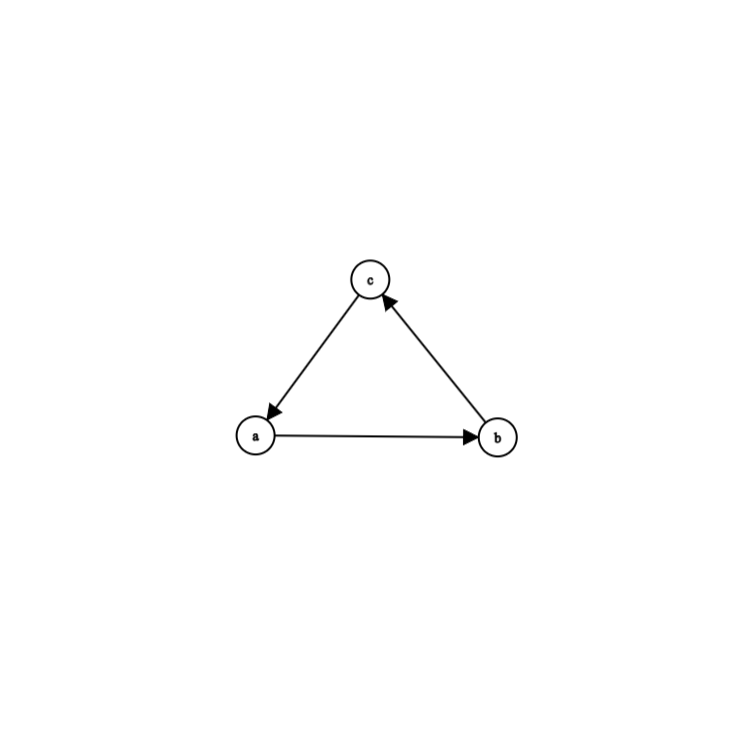
\includegraphics[width=0.4\textwidth]{Test1.png} % Replace with actual image path
\caption{Graphical representation of Test Case 1.}
\label{fig:testcase1}
\end{figure}
\item \textbf{Expected Simple Cycles:} \texttt{[[a,b,c]]}
\end{itemize}
\subsubsection{Test Case 2: Square with a Chord}
\begin{itemize}
\item \textbf{Description:} A square cycle $a \rightarrow b \rightarrow c \rightarrow d \rightarrow a$, with an additional "chord" arc $b \rightarrow d$. 
\item \textbf{Arcs Defined:}
\begin{lstlisting}[style=prologstyle, basicstyle=\ttfamily\footnotesize]
assertz(arc(1, t, a, b)).
assertz(arc(2, t, b, c)).
assertz(arc(3, t, c, d)).
assertz(arc(4, t, d, a)).
assertz(arc(5, t, b, d)). % The chord
\end{lstlisting}
\item \textbf{Graph Visualization:}
\begin{figure}[H]
\centering
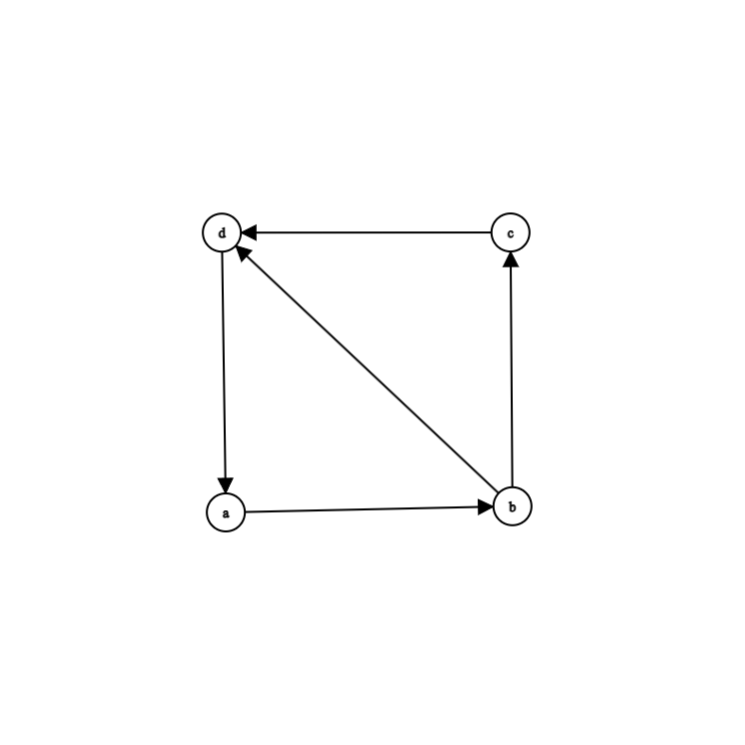
\includegraphics[width=0.5\textwidth]{Test2.png} % Replace with actual image path
\caption{Graphical representation of Test Case 2.}
\label{fig:testcase2}
\end{figure}
\item \textbf{Expected Simple Cycles:} \texttt{[[a,b,d], [b,c,d]]}. The cycle \texttt{[a,b,c,d]} (from $a \rightarrow b \rightarrow c \rightarrow d \rightarrow a$) is elementary but not simple due to the shortcut $b \rightarrow d$ (path $b \rightarrow c \rightarrow d$ has length 2, path $b \rightarrow d$ has length 1). 
\end{itemize}
\subsubsection{Test Case 3: Disjoint Cycles}
\begin{itemize}
\item \textbf{Description:} A graph containing a 2-cycle ($a \leftrightarrow b$) and two separate, non-overlapping triangles ($c \rightarrow d \rightarrow e \rightarrow c$ and $d \rightarrow f \rightarrow g \rightarrow d$). 
\item \textbf{Arcs Defined:}
\begin{lstlisting}[style=prologstyle, basicstyle=\ttfamily\footnotesize]
assertz(arc(1, t, a, b)). % 2-cycle
assertz(arc(2, t, b, a)).
assertz(arc(3, t, c, d)). % Triangle 1
assertz(arc(4, t, d, e)).
assertz(arc(5, t, e, c)).
assertz(arc(6, t, d, f)). % Triangle 2
assertz(arc(7, t, f, g)).
assertz(arc(8, t, g, d)).
\end{lstlisting}
\item \textbf{Graph Visualization:}
\begin{figure}[H]
\centering
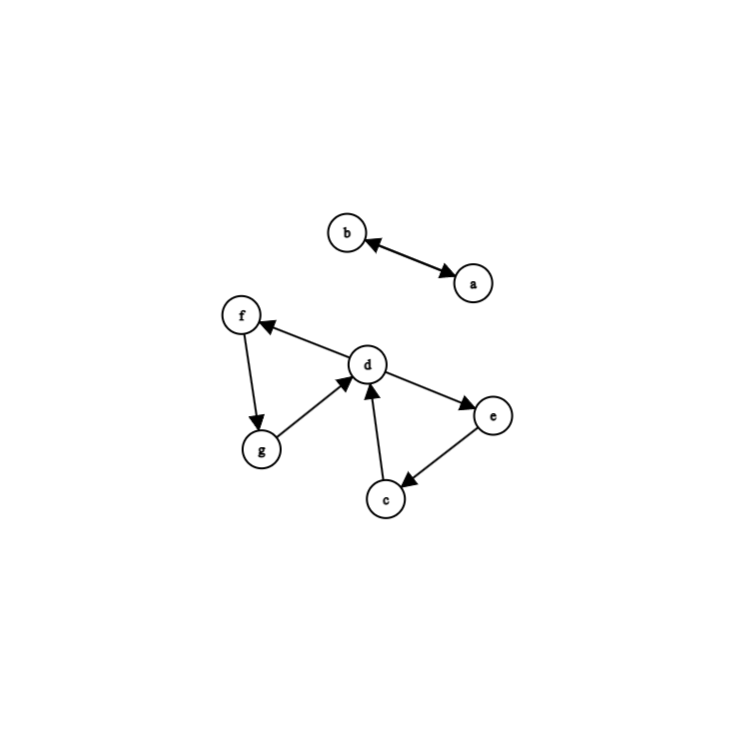
\includegraphics[width=0.7\textwidth]{Test3.png} % Replace with actual image path
\caption{Graphical representation of Test Case 3.}
\label{fig:testcase3}
\end{figure}
\item \textbf{Expected Simple Cycles:} \texttt{[[a,b], [c,d,e], [d,f,g]]} (order by \texttt{setof} might vary but content is these three).
\end{itemize}
\subsubsection{Test Case 4: Complex Overlapping Cycles and Chord}
\begin{itemize}
\item \textbf{Description:} A more complex graph with two larger, overlapping cycles and a shortcut arc.
Cycle A: $a \rightarrow b \rightarrow c \rightarrow d \rightarrow a$. 
Cycle B: $b \rightarrow e \rightarrow d \rightarrow c \rightarrow b$. 
Chord: $a \rightarrow d$. 
This also creates smaller 2-cycles like $b \leftrightarrow c$ and $c \leftrightarrow d$ due to edges from both Cycle A and Cycle B. 
\item \textbf{Arcs Defined:}
\begin{lstlisting}[style=prologstyle, basicstyle=\ttfamily\footnotesize]
assertz(arc(1, t, a, b)).
assertz(arc(2, t, b, c)).
assertz(arc(3, t, c, d)).
assertz(arc(4, t, d, a)).
assertz(arc(5, t, b, e)).
assertz(arc(6, t, e, d)).
assertz(arc(7, t, d, c)). % Edge for Cycle B, opposite of c->d in Cycle A
assertz(arc(8, t, c, b)). % Edge for Cycle B, opposite of b->c in Cycle A
assertz(arc(9, t, a, d)). % Chord for Cycle A
\end{lstlisting}
\item \textbf{Graph Visualization:}
\begin{figure}[H]
\centering
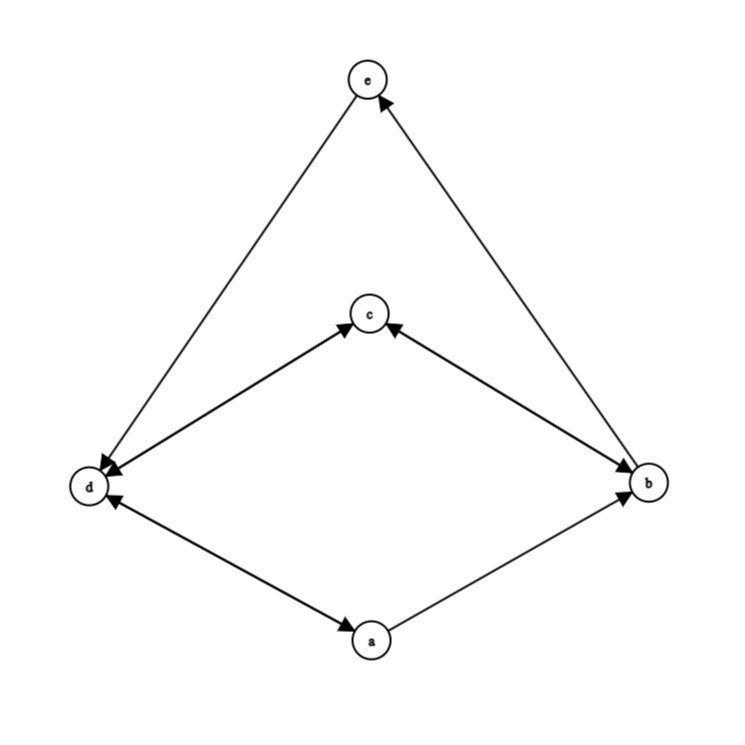
\includegraphics[width=0.6\textwidth]{Test4.png} % Replace with actual image path
\caption{Graphical representation of Test Case 4.}
\label{fig:testcase4}
\end{figure}
\item \textbf{Expected Simple Cycles:} \texttt{[[a,d], [b,c], [c,d]]}.
\begin{itemize}
\item \texttt{[a,b,c,d]} (from $a \rightarrow b \rightarrow c \rightarrow d \rightarrow a$) is not simple because path $a \rightarrow b \rightarrow c \rightarrow d$ (length 3) is longer than direct shortcut $a \rightarrow d$ (length 1). 
\item \texttt{[b,e,d,c]} (from $b \rightarrow e \rightarrow d \rightarrow c \rightarrow b$) is not simple because path $b \rightarrow e \rightarrow d \rightarrow c$ (length 3) is longer than direct shortcut $b \rightarrow c$ (length 1, via arc 2). 
\item The 2-cycles \texttt{[a,d]} ($a \rightarrow d$, $d \rightarrow a$), \texttt{[b,c]} ($b \rightarrow c$, $c \rightarrow b$), and \texttt{[c,d]} ($c \rightarrow d$, $d \rightarrow c$) are simple as their constituent 1-edge paths are inherently the shortest. 
\end{itemize}
\end{itemize}

\section{Implementazione per Grafi non Diretti}

Oltre all'algoritmo per grafi diretti descritto nelle sezioni precedenti, è stata sviluppata una variante per grafi non diretti nel file \texttt{simpleCycleUndirected.pl}. Di seguito sono descritte le principali differenze tra le due implementazioni:

\subsection{Generazione degli Archi nei Grafi non Diretti}
La principale differenza nell'implementazione per i grafi non diretti è nella generazione degli archi \texttt{edge/2} a partire dagli archi definiti tramite \texttt{arc/4}:

\begin{itemize}
\item \texttt{generate\_edges\_from\_arcs/0}: Mentre nella versione diretta ogni arco \texttt{arc(ID, Tipo, Origine, Destinazione)} genera un singolo fatto \texttt{edge(Origine, Destinazione)}, nella versione non diretta ogni arco genera due fatti: \texttt{edge(Origine, Destinazione)} e \texttt{edge(Destinazione, Origine)}, assicurandosi di evitare duplicati:

\begin{lstlisting}[style=prologstyle, basicstyle=\ttfamily\footnotesize]
generate\_edges\_from\_arcs :-
    retractall(edge(\_, \_)),
    forall(arc(\_ArcID, \_ArcType, SourceNode, DestinationNode),
           (   (   \+ edge(SourceNode, DestinationNode)
               ->  assertz(edge(SourceNode, DestinationNode))
               ;   true
               ),
               (   \+ edge(DestinationNode, SourceNode)
               ->  assertz(edge(DestinationNode, SourceNode))
               ;   true
               )
           )).
\end{lstlisting}
\end{itemize}

\subsection{Ricerca di Cicli Elementari nei Grafi non Diretti}
La procedura DFS è stata modificata per evitare cicli spuri che possono derivare dal tornare immediatamente al nodo precedente in un grafo non diretto:

\begin{itemize}
\item \texttt{dfs\_for\_cycle/4}: Nella versione per grafi non diretti, il predicate tiene traccia del predecessore immediato nel percorso e garantisce che il prossimo nodo da visitare non sia tale predecessore:

\begin{lstlisting}[style=prologstyle, basicstyle=\ttfamily\footnotesize]
dfs\_for\_cycle(CurrentNode, TargetNode, PathBackToStart, FoundCycleInReverse) :-
    PathBackToStart = [CurrentNode, Prev | \_],  % Estrae il predecessore immediato
    edge(CurrentNode, NextNode),                % Esplora un arco da CurrentNode a NextNode
    (   % Se NextNode è il target e non è il predecessore immediato, un ciclo è trovato
        NextNode == TargetNode,
        NextNode \== Prev
    ->  FoundCycleInReverse = [TargetNode | PathBackToStart]
    ;   % Altrimenti, se NextNode non è il target, assicura che non sia il predecessore immediato
        NextNode \== Prev,
        \+ memberchk(NextNode, PathBackToStart)  % Assicura che NextNode non sia già nel percorso
    ->  dfs\_for\_cycle(NextNode, TargetNode, [NextNode | PathBackToStart], FoundCycleInReverse)
    ).
\end{lstlisting}

Questo contrasta con la versione per grafi diretti, dove non è necessario escludere esplicitamente il predecessore, poiché se esiste un arco da $A$ a $B$, non necessariamente esiste un arco da $B$ a $A$:

\begin{lstlisting}[style=prologstyle, basicstyle=\ttfamily\footnotesize]
dfs\_for\_cycle(CurrentNode, TargetNode, PathBackToStart, FoundCycleInReverse) :-
    edge(CurrentNode, NextNode),
    (   NextNode == TargetNode ->
        FoundCycleInReverse = [TargetNode | PathBackToStart]
    ;   \+ memberchk(NextNode, PathBackToStart),
        dfs\_for\_cycle(NextNode, TargetNode, [NextNode | PathBackToStart], FoundCycleInReverse)
    ).
\end{lstlisting}
\end{itemize}

\subsection{Rilevamento delle Corde nei Grafi non Diretti}
La versione per grafi non diretti deve gestire in modo particolare il controllo delle corde per evitare falsi positivi:

\begin{itemize}
\item \texttt{check\_one\_node\_against\_all\_others/3}: Nella versione non diretta, il controllo salta le coppie di nodi adiacenti nel ciclo (in entrambe le direzioni) per evitare di confondere gli archi del ciclo stesso con possibili corde:

\begin{lstlisting}[style=prologstyle, basicstyle=\ttfamily\footnotesize]
check\_one\_node\_against\_all\_others(Node1, [Node2 | Rest], CycleNodes) :-
    (   Node1 == Node2
    ;   (get\_distance\_along\_cycle(Node1, Node2, CycleNodes, D1), D1 =:= 1)
    ;   (get\_distance\_along\_cycle(Node2, Node1, CycleNodes, D2), D2 =:= 1)
    )
    ->  true  % trivial: stesso nodo o adiacente nel ciclo non diretto
    ;   % Non adiacente: assicura che non esista un percorso più breve nel grafo (no corde)
        get\_distance\_along\_cycle(Node1, Node2, CycleNodes, CyclePathDistance),
        find\_shortest\_path\_length(Node1, Node2, GraphShortestDistance),
        (   GraphShortestDistance == -1
        ->  CyclePathDistance > 0  % disconnesso fuori dal ciclo
        ;   GraphShortestDistance >= CyclePathDistance
        )
    ,
    !,
    check\_one\_node\_against\_all\_others(Node1, Rest, CycleNodes).
\end{lstlisting}
\end{itemize}

\subsection{Normalizzazione dei Cicli per Grafi non Diretti}
Un ciclo in un grafo non diretto può essere percorso in entrambe le direzioni. La versione non diretta normalizza i cicli considerando entrambe le direzioni possibili:

\begin{itemize}
\item \texttt{normalize\_cycle\_representation/2}: Genera due rappresentazioni canoniche (una per ciascuna direzione di percorrenza) e sceglie la lessicograficamente minore come rappresentazione canonica:

\begin{lstlisting}[style=prologstyle, basicstyle=\ttfamily\footnotesize]
normalize\_cycle\_representation(RawReversedCycle, NormalizedNodeList) :-
    % Passo 1: Converte l'output DFS in una lista ordinata di nodi unici (CycleForward)
    RawReversedCycle = [StartNode | PathRevEnd],
    reverse(PathRevEnd, [\_StartAgain | PathForwardREST]),
    CycleForward = [StartNode | PathForwardREST],

    % Passo 2: Normalizza CycleForward iniziando dal nodo lessicograficamente minore
    find\_lexicographically\_smallest\_node(CycleForward, SmallestF),
    rotate\_list\_to\_start\_with\_element(CycleForward, SmallestF, RotFwd),

    % Passo 3: Genera e normalizza il ciclo nella direzione opposta
    reverse(CycleForward, CycleBackwardTemp),
    find\_lexicographically\_smallest\_node(CycleBackwardTemp, SmallestB),
    rotate\_list\_to\_start\_with\_element(CycleBackwardTemp, SmallestB, RotBwd),

    % Passo 4: Sceglie la lista lessicograficamente minore come rappresentazione canonica
    (  RotFwd @=< RotBwd
    -> NormalizedNodeList = RotFwd
    ;  NormalizedNodeList = RotBwd
    ).
\end{lstlisting}
\end{itemize}

Questa normalizzazione migliorata garantisce che i cicli equivalenti (percorsi in direzioni diverse) siano rappresentati in modo coerente, facilitando l'identificazione di cicli unici nei grafi non diretti.

\section{Conclusione}
Il programma Prolog implementa con successo un algoritmo per trovare i cicli semplici sia in grafi diretti che non diretti, utilizzando l'approccio descritto nelle sezioni precedenti. La versione per grafi non diretti (\texttt{simpleCycleUndirected.pl}) estende l'implementazione base (\texttt{simpleCycle.pl}) con modifiche specializzate per gestire la bidirezionalità degli archi. Entrambe le implementazioni dimostrano l'efficace uso di DFS per la rilevazione dei cicli, BFS per il calcolo dei percorsi minimi, e le capacità di Prolog per la manipolazione dinamica dei fatti e delle liste. La normalizzazione dei cicli assicura che i cicli equivalenti siano rappresentati in modo coerente e \texttt{setof/3} fornisce un elenco finale e ordinato di questi cicli semplici unici.
\end{document}